\section{光的折射}\label{sec:1-5}

在第一节里已经说过,光从一种物质进入另一种物质,它的传播方向通常会改变。
这种现象叫做光的\textbf{折射}。现在用实验来研究光的折射。

\begin{wrapfigure}[13]{r}{7cm}
    \centering
    %\includegraphics[width=7cm]{../pic/czwl2-ch1-18}
    \begin{tikzpicture}[>=Stealth, scale=0.9]
    \draw (-3, 0) -- (3, 0);
    \draw [dashed] (0, 3) -- (0, -3);
    \node at (3.7, 0) {分界面};
    \node at (-2.6, 0.4) {空气};
    \node at (-2.6, -0.4) {水};
    \node at (0.3, -0.3) {$O$};
    \node at (0.4, 2.7) {$N$};
    \node at (0.4, -2.7) {$N'$};

    \draw [rotate=50] (0, 0) -- (3, 0) [->] (2, 0) -- (1, 0);
    \draw (0, 0.8) arc [start angle=90, end angle=50, radius=0.8];
    \draw (0, 0.7) arc [start angle=90, end angle=50, radius=0.7];
    \node at (1.2, 2.0) {$A$};
    \node at (2.2, 1.5) {入射光};

    \draw [rotate=-50] (0, 0) -- (-3, 0) [->] (0, 0) -- (-1.2, 0);
    \draw (0, 0.75) arc [start angle=90, end angle=130, radius=0.75];
    \draw (0, 0.65) arc [start angle=90, end angle=130, radius=0.65];
    \node at (-2.2, 1.5) {反射光};

    \draw [rotate=60] (0, 0) -- (-3, 0) [->] (0, 0) -- (-1, 0);
    \draw (0, -0.65) arc [start angle=270, end angle=240, radius=0.65];
    \node at (-1.1, -2.4) {$B$};
    \node at (-1.9, -1.7) {折射光};
\end{tikzpicture}

    \caption{光的折射}\label{fig:1-18}
\end{wrapfigure}

让一束光从空气斜着射向水面,我们会看到,除了有一部分光反射回空气,改变了传播方向以外,
还有一部分光进入水中,也改变了传播方向(图 \ref{fig:1-18})\footnotemark。
\footnotetext{注:原书的图模糊不清,我使用 tikz 绘制了一个图片。} % 原书图片 保存为 pic 目录下的 czwl2-ch1-18.old.png

在图 \ref{fig:1-18} 里,法线是直线 $NN'$,入射角是 $\angle AON$。
折射光线 $OB$ 跟法线的夹角 $\angle BON'$ 叫做\textbf{折射角}。

在上面的实验里,如果增大或减小入射角,折射角就随着增大或减小。
但是,只要光是从空气斜射入水里,就会发生折射,并且折射角总小于入射角。

当光从水斜射入空气里的时候,也发生折射,例如光沿图 \ref{fig:1-18} 里 $BO$ 的方向从水里射到分界面上,
它就沿着 $OA$ 的方向折射。这时候折射角大于入射角。

不论光是从空气射入水里, 还是从水射入空气里,如果光是沿着法线方向入射的,通过分界面以后,
光的传播方向不改变。

从实验还可以看出,折射光线总是跟入射光线和法线在同一平面上。

如果换用别的透明物质代替水来做上面的实验,可以得到同样的结果,因此我们得到下面的结论:

\textbf{折射光线跟入射光线和法线在同一平面上,折射光线和入射光线分居在法线的两侧}。

\textbf{%
光从空气斜射入水或别的透明物质里时,折射角小于入射角;
光从水或别的透明物质斜射入空气里时,折射角大于入射角}。

在日常生活中,可以看到许多光的折射现象。
例如,插入水中的筷子,水里的部分,从水面上斜着看起来向上折了(图 \ref{fig:1-19}),就是由于光的折射的缘故。
从筷子下端 $B$ 点射出的光由水中进入空气中时,在水面处发生折射,远离法线,折射光射入眼里,
人的视觉就觉得折射光是从它的反方向延长线的 $B'$ 点发出的,$B'$ 就是 $B$ 的像。
筷子浸在水中的一段 $AB$ 上其他各点情形也是这样。因此我们就觉得整个 $AB$ 段向上折了。

\begin{figure}[htbp]
    \centering
    \begin{minipage}{7cm}
    \centering
    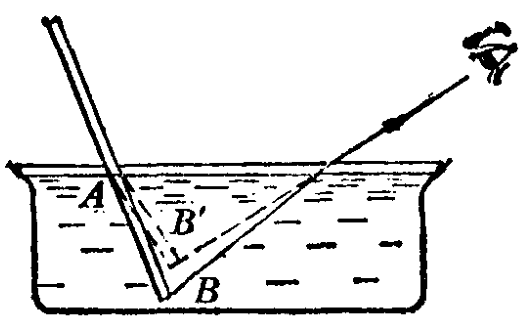
\includegraphics[width=7cm]{../pic/czwl2-ch1-19}
    \caption{插入水中的筷子变得向上弯折}\label{fig:1-19}
    \end{minipage}
    \qquad
    \begin{minipage}{7cm}
    \centering
    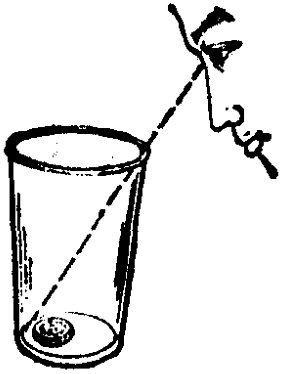
\includegraphics[width=4cm]{../pic/czwl2-ch1-20}
    \caption{}\label{fig:1-20}
    \end{minipage}
\end{figure}


\section*{小实验}

在空的茶杯里放一枚分币,移动怀子,使眼睛刚刚看不到分币(图 \ref{fig:1-20})。
保持眼睛和杯子的位置不变,慢慢地向杯里倒水。随着水面的升高,你会看到什么现象?
根据光的折射知识,对你的实验作出解释。


